\documentclass[a4paper,twoside]{article}

\usepackage[utf8]{inputenc}
\usepackage[ngerman]{babel}
\usepackage{url} %Bib
\usepackage[sort&compress,numbers]{natbib} %Bib
\usepackage{cuted}
\usepackage{epsfig}
\usepackage{subfigure}
\usepackage{calc}
\usepackage{amssymb}
\usepackage{amstext}
\usepackage{amsmath}
\usepackage{amsthm}
\usepackage{multicol}
\usepackage{pslatex}
\usepackage{apalike}
\usepackage{enumitem}
\usepackage{bbm}
\usepackage{etoolbox}
%\usepackage{hyperref}
\apptocmd{\UrlBreaks}{\do\f\do\m}{}{}
\usepackage{MOSI}     % Please add other packages that you may need BEFORE the MOSI.sty package.

\newcommand{\team}{Patrick Neher, Ruedi Lüthi}
\newcommand{\theme}{Golfstrom}
\setcounter{page}{1}

\subfigtopskip=0pt
\subfigcapskip=0pt
\subfigbottomskip=0pt

\begin{document}

	\title{Der Golfstrom\subtitle{ein einfaches mathematisches Modell} }
	
	\author{\authorname{Patrick Neher und Ruedi Lüthi}}
	
	\keywords{Golfstorm, Stabilitätsanalyse}

	\abstract{Der Golfstrom strömt. Schnell!!!!!!}
	
	\onecolumn \maketitle \normalsize \vfill

	\section{\uppercase{Der Golfstrom}}\label{sec:Golfstrom}

	\noindent Der Golfstrom ist ein Naturphänomen, welches für einen Wasseraustausch zwischen dem Golf von Mexiko und dem Nordmeer verantwortlich ist. Die Strömung beginnt jedoch nicht erst im Golf vom Mexiko sondern schon davor. Auf der Höhe des Äquator westlich von Afrika wird das Oberflächenwasser stark erwärmt, da dort die Sonne nahezu senkrecht über dem Wasser steht. Dies trägt dazu bei, dass der Albedo-Wert (wie viel Prozent der auftreffenden Strahlung reflektiert wird) klein wird und somit viel Energie in das Wasser über geht.

	Der Südost-Passat treibt dieses wärmere Wasser dann in Richtung Golf von Mexiko. Dort vereinigt sich der Strom vom Äquator mit dem Floridastrom. Ab dort Sprechen wir vom Golfstrom, den wir auch in unserem Modell betrachten. Im Golf vor Mexiko erwärmt sich das Wasser weiter bis es dann entlang der Küste Amerikas in Richtung Norden zieht. Dort spaltet sich dich Strömung und ein Teil wird von den Nordost-Passat Winden wieder Richtung Äquator gezogen und bildet einen Kreislauf. Dieser wird in unserem Modell jedoch nicht beachtet. Wir untersuchen den Teil der von der Westwindzone erfasst wird und auf dem 45 Breitengrad Richtung Europa gezogen wird.

	Dort Strömt er dann an der Norwegischen Küste weiter nach Norden. Auf dem Weg kühlt sich das warme Wasser vom Süden wieder ab und erwärmt die Luft, die dann durch die Westwinde zu uns kommt und damit unsere Temperatur stark beeinflusst. Aufgrund des Golfstromes ist unsere durchschnittliche Jahrestemperatur rund 5-10 Grad Celsius wärmer als z.B im Kanada auf dem selben Breitengrad. 

	Weiter im Norden kühlt sich das Wasser weiter ab, bis es dann anfängt zu gefrieren. Dabei wird das Salz aus dem Wasser gelöst, da dieses nicht gefriert. Deshalb steigt der Salzgehalt im nicht gefrorenen Wasser. Dies führt dazu, dass sich die Dichte des Wassers erhöht und sich deshalb absenkt. Das gesunkene Wasser fließt dann entlang der amerikanischen Küste wieder zurück zum Golf von Mexiko.

	\begin{figure}[!h]
  		\centering
 		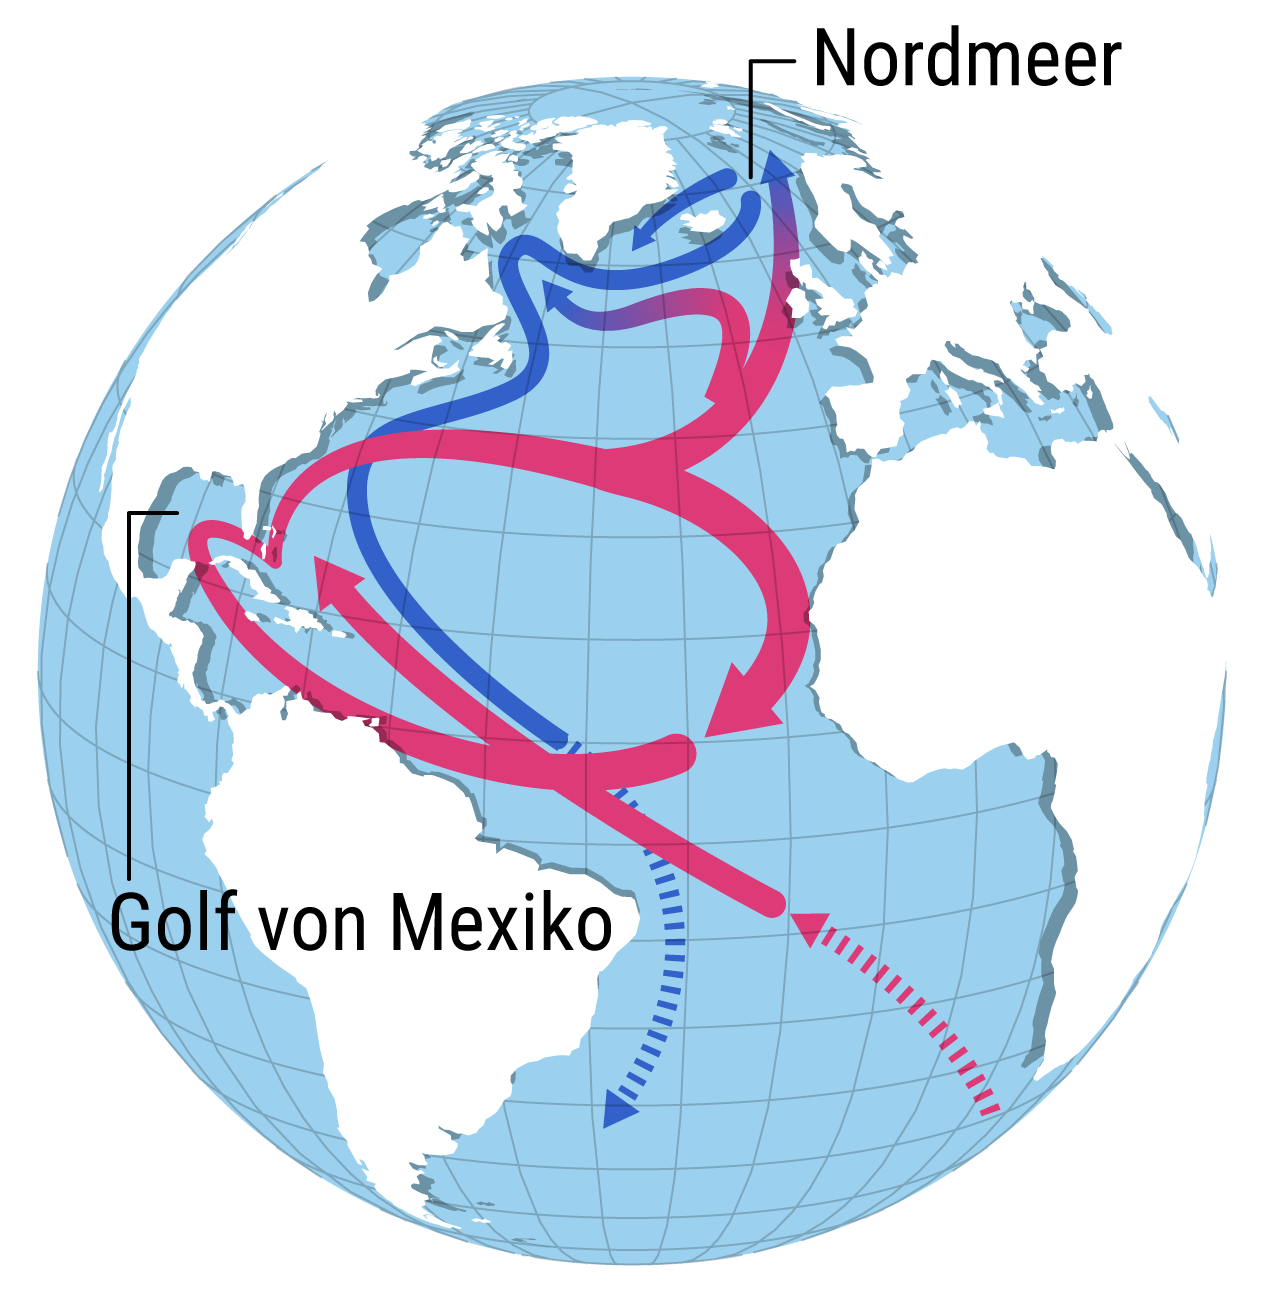
\includegraphics[width=7cm]{../Diagramme/golfstrom_fluss.png}
  		\caption{Darstellung vom Fluss des Golfstromes}
  		\label{fig:modell}
	\end{figure}

Durch den Golfstrom werden maximal 150 Millionen Kubikmeter Wasser in Bewegung gesetzt. 
Die Erwärmung der Luft ist vergleichbar mit der Leistung von Zwei Millionen modernen Atomkraftwerken. (~1.5 Petawatt)
Im Nordmeer fällt das Wasser in eine Tiefe von über 2000 Metern.
 
	

	
	\section{\uppercase{Das Modell}}\label{sec:Modell}
	
	%\noindent In dem mathematischen Modell wird von zwei Behälter ausgegangen, welche sich durch einen Fluss gegenseitig beeinflussen. Dieser Fluss beschreibt den Golfstrom: 	
	
	\noindent Das mathematische Modell besteht aus zwei Behälter \(1,2\). Diese beeinflussen sich jeweils durch den Fluss gegenseitig, gleichzeitig werden sie aber auch von konstanten Umgebungsgrößen der jeweiligen Behälter beeinflusst.
	
	\begin{figure}[!h]
  		\centering
 		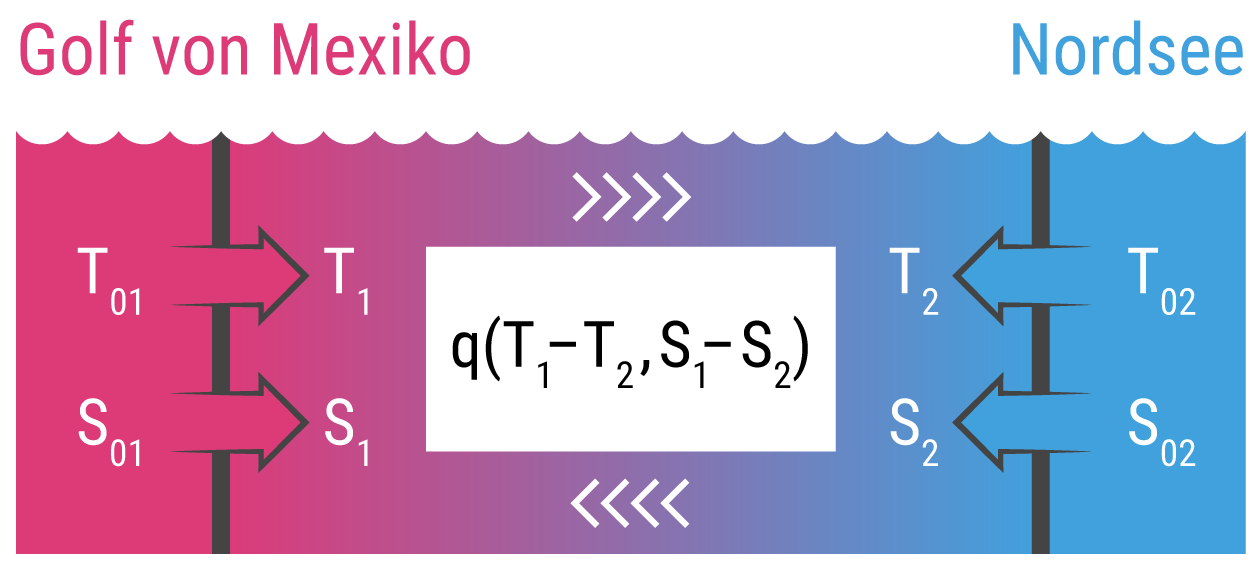
\includegraphics[width=7cm]{../Diagramme/skizze_modell.png}
  		\caption{Schematische Darstellung der zwei Behälter und des Flusses (Golfstrom) dazwischen.}
  		\label{fig:modell}
	\end{figure}
	
	Für die Indexbezeichnung der Variablen gilt in Abbildung \ref{fig:modell} sowie für das ganze nachfolgende Dokument:
	\begin{align*}
		1 &: \textrm{Golf von Mexiko} \\
		2 &: \textrm{Nordmeer}
	\end{align*}

	Jeder Behälter \(i\) hat jeweils zwei sich verändernde Variablen:
	\begin{align*}
		T_i &: \textrm{Temperatur} \\
		S_i &: \textrm{Salzgehalt}
	\end{align*}
	
	Die Umgebung der Behälter wird durch folgende Konstanten beschrieben:
	\begin{align*}
		T_{0i} &: \textrm{Temperatur der Umgebung} \\
		S_{0i} &: \textrm{Salzgehalt der Umgebung}
	\end{align*}
	
	Durch das zugrunde liegende physikalische Modell \textbf{???} wird davon ausgegangen, dass sich die Behälter langsam an die Umgebungstemperatur anpassen. Also kann die Veränderung durch die Umgebungsgrößen folgendermaßen mathematisch beschrieben werden:
	\begin{align*}
		\frac{dX_i}{dt} = k_X \left( X_{0i} - X_i \right)
	\end{align*}
	Dabei ist \(X\) die zu verändernde Größe (in unserem Modell entweder \(T\) oder \(S\)).
	Die Veränderung ist also eine Zunahme der Differenz zwischen aktuellem Wert und dem Wert der Umgebung multipliziert mit einer Austauschkonstante \(k_X\).
	
	Wiederum aus dem physikalische Modell ist bekannt, dass die Veränderung durch den Fluss \(q\) sich proportional zur Differenz der Dichte der beiden Behälter beschreiben lässt:
	\begin{align*}
		q = a \left( \rho_2 - \rho_1 \right)
	\end{align*}
	Wie viel Meereswasser nun zwischen den zwei Behälter hin und her fließt, unterliegt sicherlich noch weiteren Umwelteinflüssen. Diese werden in der Konstante \(a\) zusammengefasst.
	
	Die Dichte ist abhängig von Temperatur und Salzgehalt des Meereswasser. Dieser Zusammenhang wird hier vereinfacht als linear angenommen:
	\begin{align*}
		\rho_i = \rho_0 - bT_i + cS_i
	\end{align*}
	
	Die Konstanten \(b\) und \(c\) sind also unveränderliche Naturkonstanten.
	
	Setzt man den Zusammenhang für die Dichte in die Gleichung für den Fluss ein:
	\begin{align*}
		q &= a \left( \rho_0 - bT_2 + cS_2 - \left( \rho_0 - bT_1 + cS_1 \right) \right) \\
		&= a \left( b\left( T_1 - T_2 \right) - c \left( S_1 - S_2 \right) \right)
	\end{align*}
	So wird ersichtlich, dass für den Fluss die Referenzdichte \(\rho_0\) keinen Einfluss hat.
	
	Alles zusammengesetzt ergibt für die vier veränderlichen Größen folgendes Gleichungssystem:
	\begin{align*}
		\frac{dT_1}{dt} &= k_T\left(T_{01} - T_1\right) + \left|q(T_1 - T_2,S_1 - T_2)\right|\left(T_2 - T_1\right) \\
		\frac{dT_2}{dt} &= k_T\left(T_{02} - T_2\right) + \left|q(T_1 - T_2,S_1 - T_2)\right|\left(T_1 - T_2\right) \\
		\frac{dS_1}{dt} &= k_S\left(S_{01} - S_1\right) + \left|q(T_1 - T_2,S_1 - T_2)\right|\left(S_2 - S_1\right) \\
		\frac{dS_2}{dt} &= k_S\left(S_{02} - S_2\right) + \left|q(T_1 - T_2,S_1 - T_2)\right|\left(S_1 - S_2\right)
	\end{align*}
	 
	 In den Gleichungen treten die abhängigen Größen jeweils immer als Differenz der beiden Behälter auf. Also kann das Modell so umgeschrieben werden, dass es nur noch von den Differenzen abhängt. Sei \(T = T_1 - T_2, T_0 = T_{01} - T_{02}\) und \(S = S_1 - S_2, S_0 = S_{01} - S_{02}\)  so ist:
	 \begin{align*}
	 	\frac{dT}{dt} = \frac{dT_1}{dt} - \frac{dT_2}{dt} &= k_T\left(T_{0} - T\right) - 2\left|q(T,S)\right|T \\
	 	\frac{dS}{dt} = \frac{dS_1}{dt} - \frac{dS_2}{dt} &= k_S\left(S_{0} - S\right) - 2\left|q(T,S)\right|S \\
	 	q(T,S) &= a\left(bT - cS\right)
	 \end{align*}
	  
	Aus der Realität \textbf{???} ist bekannt, dass die Umgebungstemperatur \(T_1\) im Golf von Mexiko höher ist als im Nordmeer \(T_2\). Auch bekannt ist, dass der Salzgehalt \(S_1\) im Golf tiefer ist als im Nordmeer \(S_2\). Es gilt also:
	\begin{align*}
		T_1 > T_2 \quad \textrm{und} \quad S_1 < S_2
	\end{align*}
	
	Diese Bedingungen sind in einer ersten Simulation in Abbildung \ref{fig:modell_q_pos}  dargestellt. Klar zu erkennen ist, dass sich bereits nach nur kurzer Zeit für den Fluss einen stabilen Zustand einstellt. Der Fluss stellt sich zum Ende bei \(0.45\), also fließt Wasser vom Golf von Mexiko über die Oberfläche in das Nordmeer und im Untergrund wieder zurück.
	
	\begin{figure}[!h]
  		\centering
 		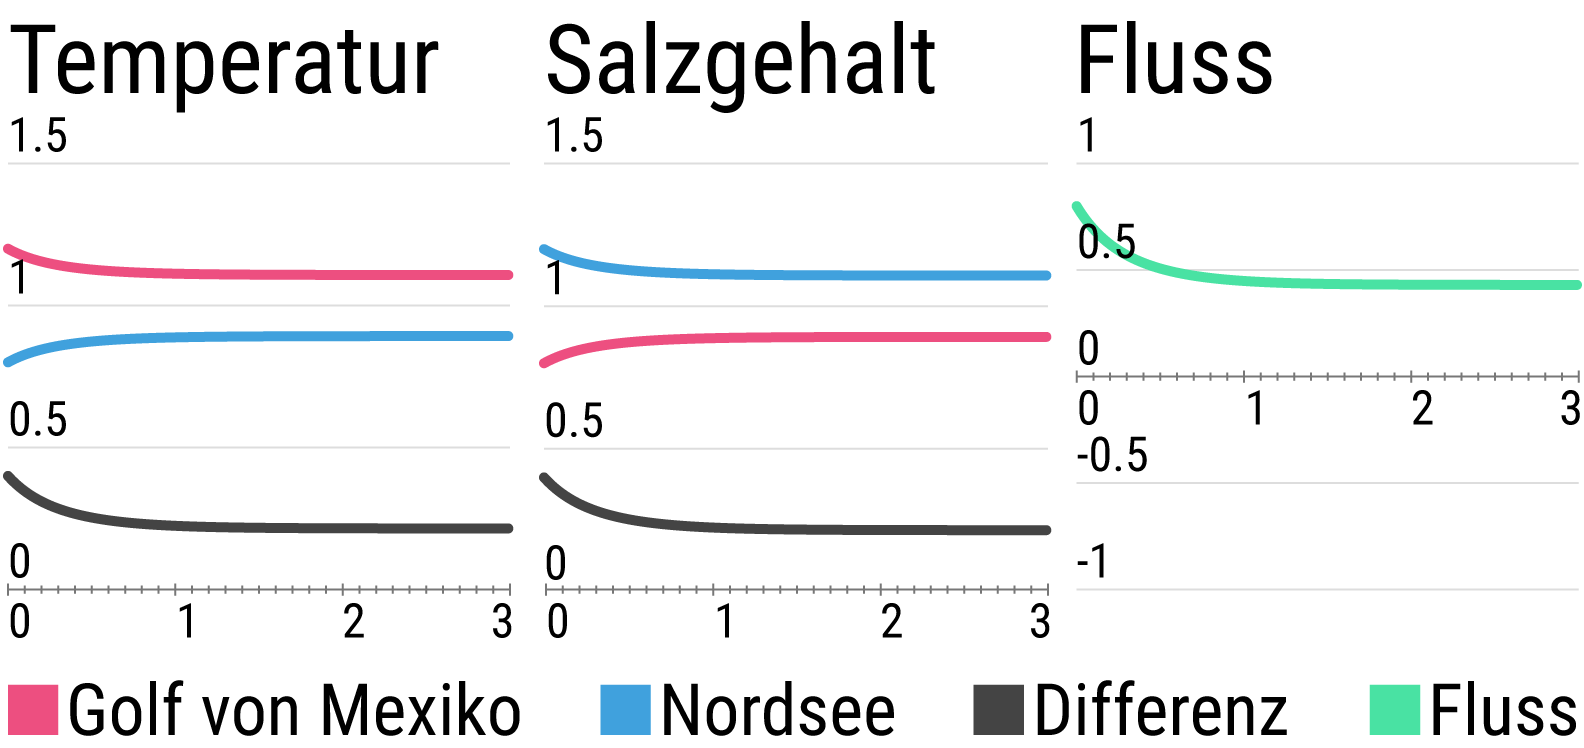
\includegraphics[width=7cm]{../Diagramme/temp-salt-flow_q-pos.png}
  		\caption{Simulation mit folgenden theoretischen Werten \(T_{01} = S_{02} = 1.2, T_{02} = S_{01} = 0.8, k_T = k_S = 1, a = b = c = 1\)}
  		\label{fig:modell_q_pos}
	\end{figure}
	
	Sinkt der Salzgehalt im Nordmeer durch äußere Einflüsse, so ergibt sich ein verändertes Bild. In Abbildung \ref{fig:modell_q_neg} hat der Fluss ein negatives Vorzeichen, er hat sich also umgedreht. Das Wasser fließt neu in entgegengesetzter Richtung vom Nordmeer in den Golf von Mexiko.
	\begin{figure}[!h]
  		\centering
 		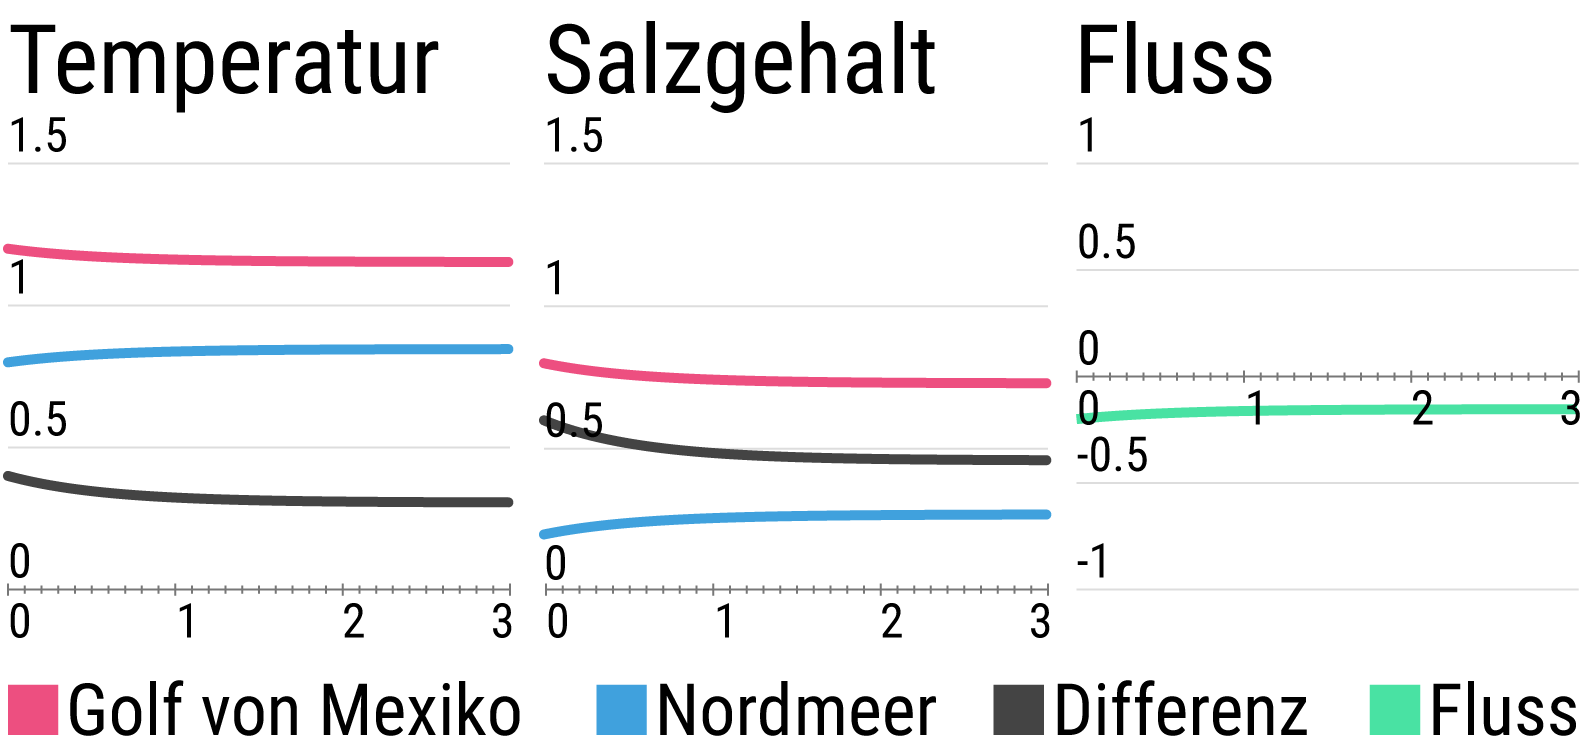
\includegraphics[width=7cm]{../Diagramme/temp-salt-flow_q-neg.png}
  		\caption{Erneute Simulation mit tiefem Salzgehalt \(S_2 = 0.2\) im Nordmeer (die anderen Parameter wurden wie in Abbildung \ref{fig:modell_q_pos} beibehalten)}
  		\label{fig:modell_q_neg}
	\end{figure}
	
	\subsection{Entdimensionalisierung}
	Da die Dimensionen (oder Maßeinheiten) für das Verhalten des Modells keine Rolle spielen, werden diese in einem nächsten Schritt rausgekürzt. Dies geschieht durch die Wahl einer geeigneten Skalierung. Diese ergibt sich, indem wir das Modell nur von dem Verhältnis zu den jeweiligen Startwerten \(T_0, S_0\) abhängig machen. Sei also:
	\begin{align*}
		\tilde{T} = \frac{T}{T_0} \Rightarrow T = \tilde{T} T_0 \quad \textrm{und} \quad \tilde{S} = \frac{S}{S_0} \Rightarrow S = \tilde{S} S_0
	\end{align*}
	
	Eingesetzt in die Gleichung für die Temperaturdifferenz ergibt sich folgendes:
	\begin{align*}
		\frac{d\tilde{T} T_0}{dt} &= k_T\left(T_{0} - \tilde{T} T_0 \right) - 2\left|q(\tilde{T} T_0,\tilde{S} S_0)\right| \tilde{T} T_0 \\
		\stackrel{
			\substack{
				\textrm{da } T_0 > 0\\
				\textrm{ist } T_0 \neq 0
			}
		}{\Rightarrow}
		\frac{d\tilde{T}}{dt} &= k_T\left(1 - \tilde{T}\right) - 2\left|q(\tilde{T} T_0,\tilde{S} S_0)\right| \tilde{T}
	\end{align*}
	Analog gilt für den Salzgehalt:
	\begin{align*}
		\frac{d\tilde{S}}{dt} &= k_S\left(1 - \tilde{S}\right) - 2\left|q(\tilde{T} T_0,\tilde{S} S_0)\right| \tilde{S}
	\end{align*}
	Gilt zusätzlich für den Fluss:
	\begin{align*}
		q = \frac{\tilde{q} k_T}{2} &= a \left( b\tilde{T}T_0 - c\tilde{S}S_0 \right) \\
		\Rightarrow \tilde{q} &= \underbrace{2\frac{ab}{k_T}T_0}_{= \alpha} \cdot \tilde{T} - \underbrace{2\frac{ac}{k_T}S_0}_{=\beta} \cdot \tilde{S} \\
		\Rightarrow \tilde{q} &= \alpha\tilde{T} - \beta\tilde{S}
	\end{align*}
	Skalieren wir zusätzlich noch die Zeit \(t = \tilde{t} k_T\) und setzen \(q = \frac{\tilde{q}k_T}{2}\) ein, so gilt für die Temperatur:
	\begin{align*}
		\frac{d\tilde{T}}{d\tilde{t} k_T} &= k_T\left(1 - \tilde{T}\right) - 2\left|\frac{\tilde{q}(\tilde{T},\tilde{S})k_T}{2}\right| \tilde{T} \\
		\Rightarrow \frac{d\tilde{T}}{d\tilde{t}} &= (1 - \tilde{T}) - \left| \tilde{q}(\tilde{T},\tilde{S})\right|\tilde{T}
	\end{align*}
	Wiederum analog für den Salzgehalt gilt:
	\begin{align*}
		\Rightarrow \frac{d\tilde{S}}{d\tilde{t}} &= \underbrace{\frac{k_S}{k_T}}_{=\gamma}(1 - \tilde{S}) - \left| \tilde{q}(\tilde{T},\tilde{S})\right|\tilde{S}
	\end{align*}
	
	Für die nachfolgende Gleichgewichtsuntersuchung wird nur das dimensionslose Modell betrachtet. Um dafür die Bezeichnungen der Variablen einfach zu halten, wird auf die zusätzliche Notation mit dem \textasciitilde\ verzichtet. Also lauten die dimensionslosen Gleichungen nun:
	\begin{align*}
		\frac{dT}{dt} &= (1 - T) - \left| q(T,S)\right|T \\
		\frac{dS}{dt} &= \gamma (1 - S) - \left| q(T,S)\right|S \\
		q(T,S) &= \alpha T - \beta S
	\end{align*}
	Dafür wurden folgenden Parameter definiert:
	\begin{align*}
		\alpha = 2\frac{ab}{k_T}T_0 \qquad
		\beta = 2\frac{ac}{k_T}S_0 \qquad
		\gamma = \frac{k_S}{k_T}
	\end{align*}
	
	\subsection{Gleichgewichtsuntersuchung}
	Das System ist im Gleichgewicht, wenn sich Temperatur und Salzgehalt nicht mehr ändert:
	\begin{align*}
		\frac{dT}{dt} = (1 - T) - \left| q(T,S)\right|T &\stackrel{!}{=} 0 \\
		\Rightarrow 1 - T(1 + |q|) &\stackrel{!}{=} 0 \\
		\Rightarrow T &= \frac{1}{1 + |q|} \\
		\stackrel{
			\substack{
				\textrm{analog für den}\\
				\textrm{Salzgehalt}
			}
		}{\Rightarrow} S &= \frac{\gamma}{\gamma + |q|}
	\end{align*}
	Damit ist der Fluss:
	\begin{align*}
		q = \alpha \frac{1}{1 + |q|} - \beta \frac{\gamma}{\gamma + |q|} = g(q)
	\end{align*}
	Diesen Zusammenhang bezeichnen wir für die weiteren Untersuchungen als Funktion \(g(q)\).
	
	Wenn sich der Fluss nicht mehr ändert, also stabil ist, muss für \(g(q)\) folgendes gelten:
	\begin{align*}
		g(q) \stackrel{!}{=} q \Rightarrow q - g(q) \stackrel{!}{=} 0
	\end{align*}
	Um also den Fluss im stabilen Zustand zu bestimmen, müssen entsprechende Nullstellen gefunden werden. Im Fall \(\gamma = 1\) und \(q \neq 0\) können die Nullstellen direkt ausgerechnet werden:
	\begin{align*}
		g(q) = q - \frac{1}{1 + |q|}  \left(\alpha - \beta\ \right) &\stackrel{!}{=} 0 \\
		\Rightarrow \frac{q \left( 1 + |q| \right)}{1 + |q|} + \frac{\beta - \alpha}{1 + |q|}  &\stackrel{!}{=} 0 \\
		\stackrel{\textrm{da } 1 + |q| > 0}{\Rightarrow} \left. \begin{array}{ll}
			q > 0: & q^2 + q + \beta - \alpha \\
			q < 0: & -q^2 - q + \beta - \alpha
		\end{array} \right\} &\stackrel{!}{=} 0 \\
		\Rightarrow \begin{array}{l}
			q > 0 \left\{ \begin{array}{l}
				q_1 = \frac{1}{2}\left( -\sqrt{4a - 4b + 1} -1 \right)	\\			
				q_2 = \frac{1}{2}\left( +\sqrt{4a - 4b + 1} -1 \right)				
			\end{array}\right. \\
			q < 0 \left\{ \begin{array}{l}
				q_3 = \frac{1}{2}\left( -\sqrt{4b - 4a + 1} + 1 \right) \\
				q_4 = \frac{1}{2}\left( +\sqrt{4b - 4a + 1} + 1 \right)
			\end{array}\right.
		\end{array}
	\end{align*}
	Da \(q_1\) für reelle Werte die Bedingung \(q > 0\) nicht erfüllt, kann es keine Nullstelle sein. Auch \(q_4\) kann für reelle Werte die Bedingung \(q < 0\) nicht erfüllen. Also verbleiben für den Fall \(\gamma = 1\) die Nullstellen \(q_2\) und \(q_3\).
	
	\begin{figure}[!h]
  		\centering
 		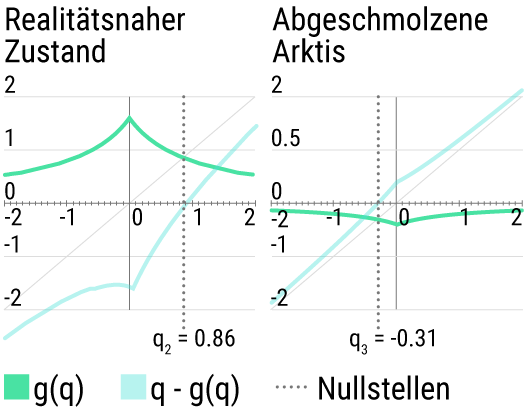
\includegraphics[width=6cm]{../Diagramme/g_von_q_gamma_1.png}
  		\caption{Die Funktion \(g(q)\) mit den Nullstellen \(q_2\) und \(q_3\) für die bereits beschriebenen Werte im realitätsnahen Zustand (siehe Abbildung \ref{fig:modell_q_pos}) und im Fall einer abgeschmolzenen Arktis (siehe Abbildung \ref{fig:modell_q_neg}).}
  		\label{fig:g_von_q_gamma_1}
	\end{figure}	

	
	Um auch den Fall \(\gamma \neq 1\) betrachten zu können, wird die Funktion \(g(q)\) so erweitert, dass die Brüche wegfallen aber die Nullstellen erhalten bleiben:
	\begin{align*}
		k(q) = \left\{ \begin{array}{ll}
			\left( q - g\left(q\right) \right)(1 + q)(\gamma + q) &\textrm{ für } q > 0  \\
			\left( g\left(q\right) - q \right)(1 - q)(\gamma - q) &\textrm{ für } q < 0
		\end{array} \right.
	\end{align*}
	Aufgrund der Betragsfunktion für \(q\) in der Funktion \(g(q)\) müssen wir die Fälle \(q > 0\) und \(q < 0\) getrennt betrachten. 
	
	\noindent\underline{Fall 1} \((q > 0):\)
	\noindent Eingesetzt und ausmultipliziert ergibt sich folgendes Polynom:
	\begin{align*}
		k_{q>0}(q) &= q^3 + q^2(1 + \gamma) + q\left(\gamma \left(1 + \beta\right) - \alpha \right) + \gamma \left( \beta - \alpha \right)
	\end{align*}
	Die Funktion \(k(q)\) ist ein Polynom 3ten Grades und hat höchstens drei Nullstellen. Diese drei Nullstellen müssen wiederum zwei Wendepunkte einschließen. Die Wendepunkte werden wie folgt gefunden:
	\begin{align*}
		&k_{q>0}'(q) = 3q^2 + 2q(1+\gamma) + \gamma(1+\beta) - \alpha \stackrel{!}{=} 0 \\
		&\Rightarrow \left\{ \begin{array}{l}
			q_{w1} = -\frac{1}{3}\left( \sqrt{3\alpha - 3\beta\gamma + \gamma^2 - \gamma + 1} +\gamma + 1 \right) \\
			q_{w2} = \frac{1}{3}\left( \sqrt{3\alpha - 3\beta\gamma + \gamma^2 - \gamma + 1} -\gamma - 1 \right)
		\end{array} \right.
	\end{align*}
	Der Wendepunkt \(q_{w1}\) kann für reelle Werte nicht größer Null sein und ist für den Fall \(q > 0\) also nicht relevant. Somit hat \(k(q)\) für \(q > 0\) nur den Wendepunkt \(q_{w2}\) und kann damit auch nur zwei Nullstellen im Bereich \(q > 0\) haben.
	
	Gilt \(k(q_{w2}) = 0\) so ist gerade der Wendepunkt ein Nullpunkt und die Funktion \(k(q)\) hat eine Nullstelle für \(q > 0\).
	
	Ist \(q_{w2} < 0\) oder ist \(k(0) > 0\) und \(k(q_{w2}) > 0\) so existiert für \(q > 0\) keine Nullstelle, so beispielsweise im Fall der abgeschmolzenen Arktis.
	
	\noindent\underline{Fall 2} \((q < 0):\) Analog zum Fall 1 kann auch in diesem Bereich jeweils nur ein Wendepunkt sein. Dies bedeutet, dass auch hier nur höchstens zwei Nullstellen liegen.
	
	\begin{figure}[!h]
  		\centering
 		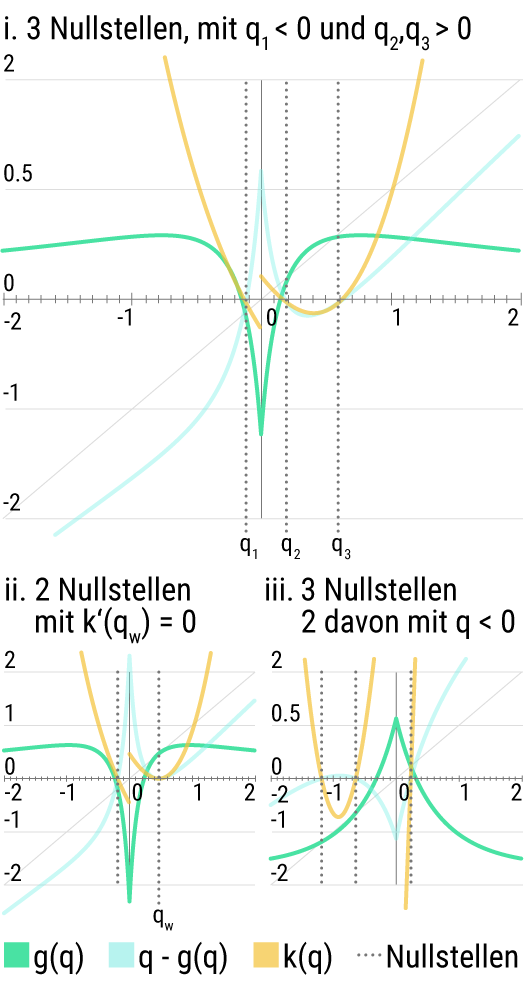
\includegraphics[width=6cm]{../Diagramme/q_von_q_falluntersuchung_anderes_layout.png}
  		\caption{Gleichgewichtsbestimmung mittels der Funktion \(k(q)\) für 3 verschiedene Beispiele. Das Beispiel i. ist durch die Parameter \(T_{01} = S_{01} = 2, T_{02} = 0.8, S_{02} = 0.2, k_T = 1, k_S = 0.2, a = b = c = 1 \) bestimmt und hat die Nullstellen \(q_1 \approx -0.1, q_2 \approx 0.2, q_3 \approx 0.6\). }
  		\label{fig:q_von_q_falluntersuchung}
	\end{figure}	
	
	\subsection{Stabilitätsanalyse}
	Sei
	\begin{align*}
		\nabla f = \left(\begin{array}{c}
			f_T \\
			f_S
		\end{array}\right) = \left(\begin{array}{c}
			1 - T - |\alpha T - \beta S|T \\
			\gamma - \gamma S - |\alpha T - \beta S|S
		\end{array}\right)
	\end{align*}
	der Gradient unseres dimensionslosen Modells. Linearisieren wir nun diesen um unsere Gleichgewichtspunkte und es entsteht folgende Jacobi-Matrix:
	\begin{align*}
		Df &= \left(\begin{array}{cc}
			\frac{\partial f_T}{\partial T} & \frac{\partial f_T}{\partial S} \\
			\frac{\partial f_S}{\partial T} & \frac{\partial f_S}{\partial S} \\
		\end{array}\right)
	\end{align*}
	mit
	\begin{align*}
		\frac{\partial f_T}{\partial T} &= -1 - \frac{\alpha T - \beta S}{|\alpha T - \beta S|}\alpha T - |\alpha T - \beta S| \\
		 \frac{\partial f_T}{\partial S} &= -\frac{\alpha T - \beta S}{|\alpha T - \beta S|}(-\beta) T \\
		 \frac{\partial f_S}{\partial T} &= -\frac{\alpha T - \beta S}{|\alpha T - \beta S|}\alpha S \\
		 \frac{\partial f_S}{\partial S} &= -\gamma -\frac{\alpha T - \beta S}{|\alpha T - \beta S|}(-\beta) S - |\alpha T - \beta S|
	\end{align*}
	Setzen wir für \(\alpha T - \beta S = q\) ein und betrachten das charakteristische Polynom:
	\begin{align*}
		&P_{Df}(\lambda) = \textrm{det}\left( Df - \lambda  \mathbbm{1} \right) = \\
		&\left(-1 - \frac{q}{|q|}\alpha T - |q| - \lambda\right) \cdot \left( -\gamma - \frac{q}{|q|}(-\beta) S - |q|- \lambda \right)\\
		& - \frac{q}{|q|}\alpha S \cdot  \frac{q}{|q|}(-\beta) T = 
		\lambda^2 + \lambda \underbrace{\left( 1  + \gamma + 2|q| + \frac{q^2}{|q|} \right)}_{-\textrm{spur}(Df) > 0 ~\Rightarrow~ \textrm{spur}(Df) < 0} + \\
		& \underbrace{
			\underbrace{\frac{q}{|q|}\left(\alpha T \gamma - \beta S + \alpha T |q| - |q|\beta S\right)}_{:=h(q)}
			 + \underbrace{\gamma + |q| + |q|\gamma + |q|^2}_{=(1 + |q|)(\gamma + |q|)}
		}_{\textrm{det}(Df)}
	\end{align*}
	Untersuchen wir die Determinante \(\textrm{det}(Df)\) weiter:
	\begin{align*}
		\textrm{det}(Df) = (1 + |q|)(\gamma + |q|)\left( 1 + \underbrace{\frac{h(q)}{(1 + |q|)(\gamma + |q|)}}_{:=h^*(q)} \right)
	\end{align*}
	Betrachten wir die Funktion \(h(q)\) etwas genauer und setzen für \(T = \frac{1}{1+|q|}, S = \frac{\gamma}{\gamma + |q|}\) ein:
	\begin{align*}
		h(q) &= \frac{q}{|q|}\left(
			\frac{\alpha \gamma}{1 + |q|} - \frac{\beta \gamma}{\gamma + |q|} + 
			\frac{|q| \alpha}{1+|q|} - \frac{|q| \beta\gamma}{\gamma + |q|}
		\right) \\
		&=\frac{q}{|q|}\left(
			\frac{\alpha}{1 + |q|}(\gamma + |q|) -
			 \frac{\beta \gamma}{\gamma + |q|}(1+|q|)
		\right)
	\end{align*}
	Setzen wir nun dieses Resultat in die Funktion \(h^*(q)\) ein:
	\begin{align*}
		h^*(q) &= \frac{q}{|q|}\left(
			\frac{\frac{\alpha}{1 + |q|}(\gamma + |q|) -
			 \frac{\beta \gamma}{\gamma + |q|}(1+|q|)}
			{(1 + |q|)(\gamma + |q|)}
		\right) \\
		&= \frac{q}{|q|} \left(
			\frac{\alpha}{(1+|q|)^2} - \frac{\beta \gamma}{(\gamma + |q|)^2}
		\right)
	\end{align*}
	Dies entspricht gerade bis auf das Vorzeichen der folgender Ableitung:
	\begin{align*}
		g'(q) &= \frac{d}{dq} \left(\alpha\frac{1}{1+|q|} - \beta\frac{\gamma}{\gamma+|q|}\right) \\
		&= -\frac{q}{|q|} \frac{\alpha}{(1+|q|)^2} + \frac{q}{|q|} \frac{\beta \gamma}{(\gamma + |q|)^2}
	\end{align*}
	Also gilt für die Determinante \(\textrm{det}(Df)\):
	\begin{align*}
		\textrm{det}(Df) = \underbrace{(1+|q|)(\gamma+|q|)}_{> 0}(1-g'(q))
	\end{align*}
	Über die Eigenschaften der Spur lassen sich nun folgende Aussagen über die Eigenwerte \(\lambda_1, \lambda_2\) treffen:
	\begin{align*}
		\textrm{spur}(Df) < 0 \quad &\Rightarrow \quad  \lambda_1 + \lambda_2 < 0 \\
	\end{align*}
	Also dürfen nicht beide Eigenwerte \(\lambda_1, \lambda_2\) positiv sein und somit ist mindestens einer oder beide negativ. \\
	Über die Determinante wissen wir:
	\begin{align*}
		\textrm{det}(Df) = \lambda_1 \cdot \lambda_2 \left\{ \begin{array}{l}
			> 0 \textrm{ wenn } g'(q) < 1 \\
			< 0 \textrm{ wenn } g'(q) > 1
		\end{array} \right.
	\end{align*}
	Also ist ein Gleichgewichtspunkt \(q_i\) stabil wenn \(g'(q_i) < 1\), denn dann müssen ja beide Eigenwerte \(\lambda_1, \lambda_2\) negativ sein. Ansonsten wären die Bedingungen für die \(\textrm{spur}(Df)\) und \(\textrm{det}(Df)\) verletzt. Gilt hingegen\(g'(q_i) > 1\) ist der Gleichgewichtspunkt instabil.
	
	\begin{figure}[!h]
  		\centering
 		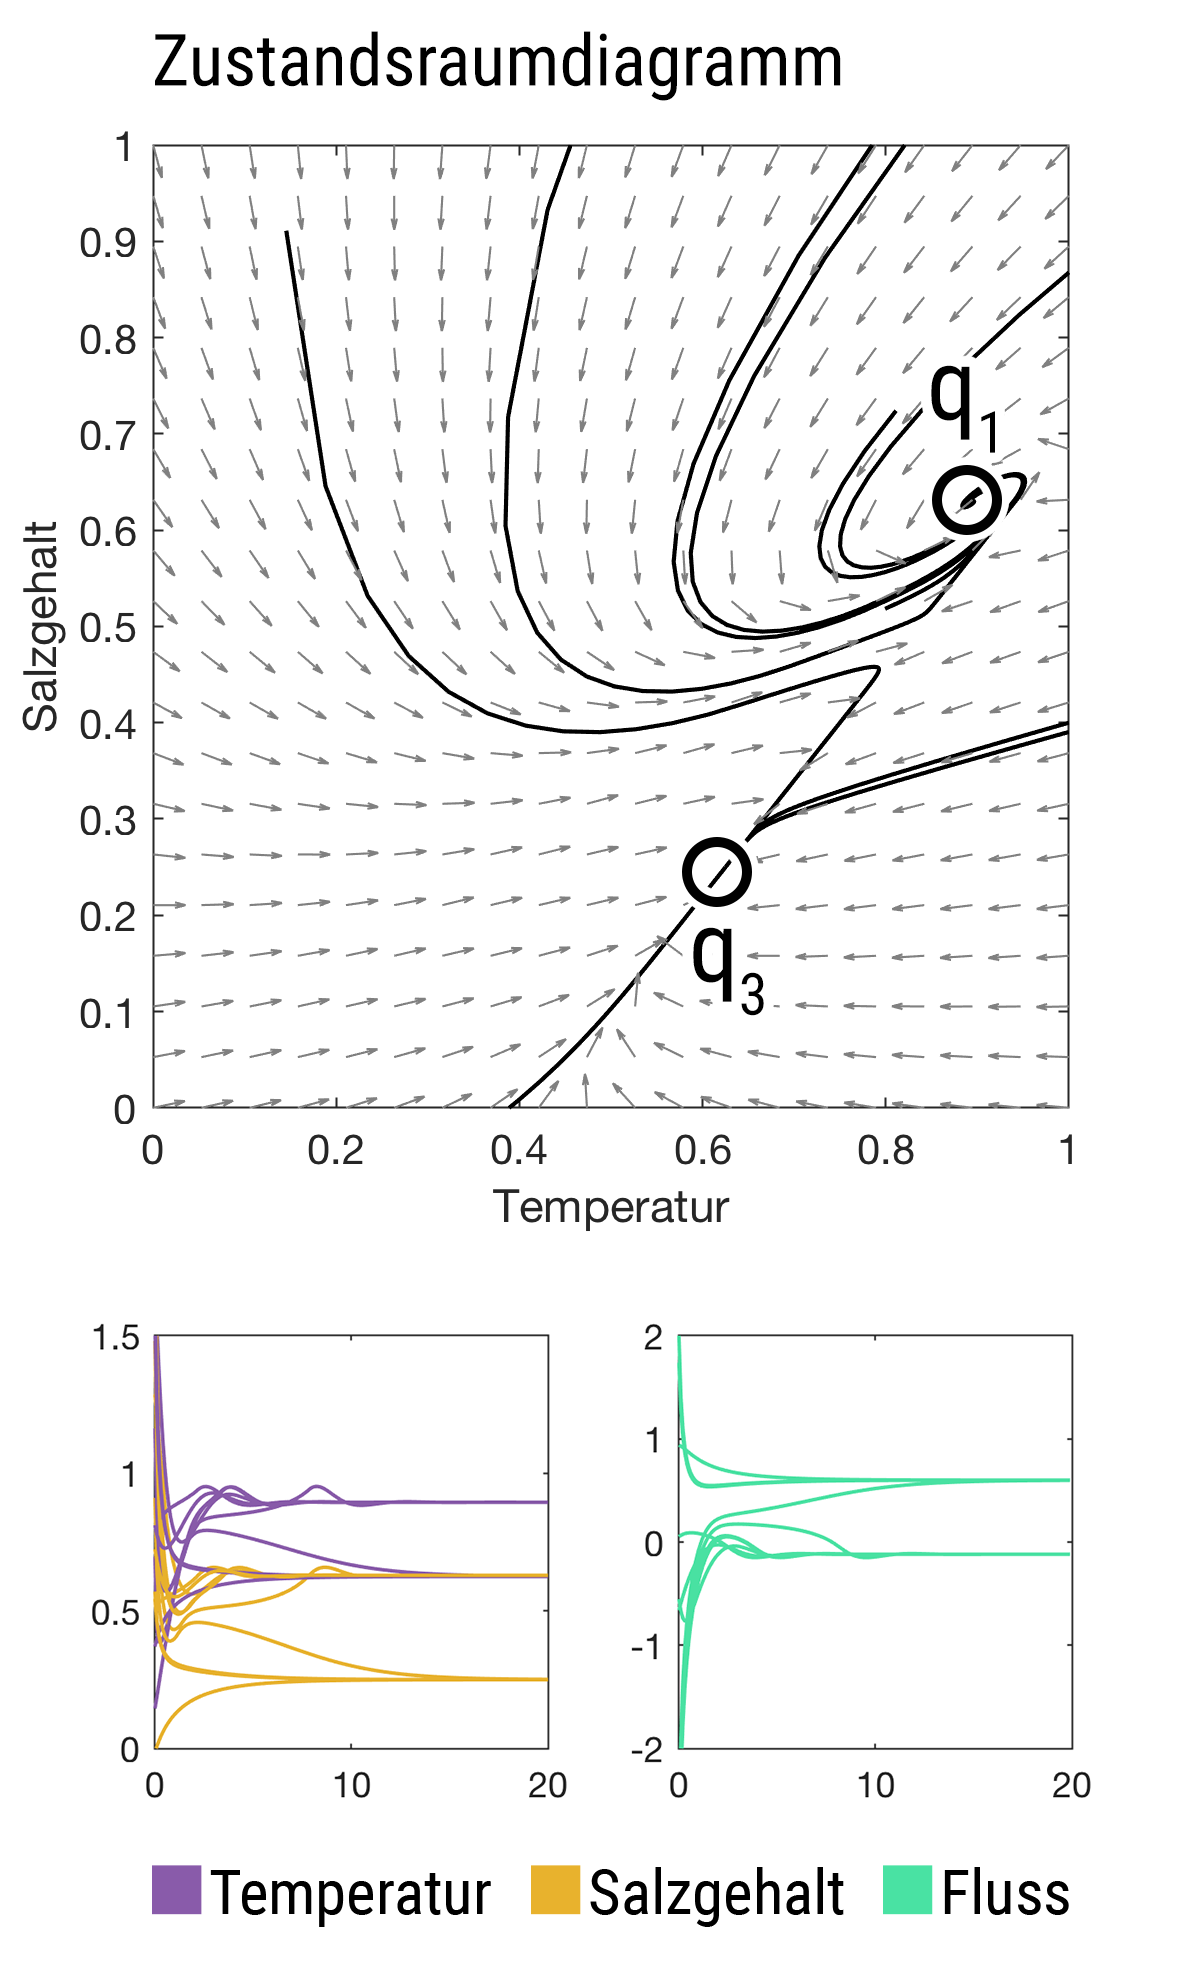
\includegraphics[width=7cm]{../Diagramme/zustandsdiagram.png}
  		\caption{Zustandsraumdiagram für das Beispiel i. aus Abbildung \ref{fig:q_von_q_falluntersuchung}. Für den Plot wurden zufällige Startwerte für \(T\) und \(S\) gewählt. Aus der Ableitung \(g'\) wissen wir ob es sich um stabile oder instabile Punkte handelt: \(g'(q_1) \approx -5.4 < 1 \Rightarrow \textrm{stabil}, g'(q_2) \approx 2.8 > 1 \Rightarrow \textrm{instabil}, g'(q_3) \approx 0.2 \Rightarrow < 1 \Rightarrow \textrm{stabil} \). }
  		\label{fig:Zustandsraumdiagram}
	\end{figure}	
	
	\section{\uppercase{Anwendung}}\label{sec:Anwendung}
	\noindent Nach der theoretischen Analyse wollen wir unser Modell welches noch nicht enddimensioniert wurde betrachten. Dazu haben wir recherchiert und die tatsächlichen Temperaturen des Golfstrom genommen. Da sich die Quellen jedoch unterscheiden, da in verschieden Tiefen gemessen wurde oder zu verschieden Jahreszeiten oder die Genauigkeit der Messung variiert haben wir uns dazu entschieden ein Mittel der Werte zu nehmen.
	
	\subsection{Datenabschätzung}
	\noindent Betrachten wir nun zuerst die Temperaturen des Golfstromes im Golf von Mexiko. Der Golf von Mexiko hat eine durchschnittliche Temperatur von ungefähr 27 Grad Celsius. An manchen Küstenabschnitten etwas wärmer an anderen etwas kühler. An der Küste wird der Golfstrom in seinem Fluss gestört, da dort der Meeresgrund nicht überall gleich tief ist. So kommt es dazu, dass der Fluss an mancher Stelle durch eine enge muss und sich somit die Fließgeschwindigkeit erhöht und an andere Stelle wird er wieder gebremst. Dadurch verweilt die Wassermenge an einer Stelle länger und wird stärker von der Sonne erwärmt. 
	
	Die Temperatur vom Nordmeer haben wir mit rund 10 Grad Celsius angenommen. Hierbei ist es schwer, da das Nordmeer relativ groß ist und sich über circa 15 Breitengrade erstreckt. Das ist eine Länge von über 2000 Kilometern. Auf dieser enormen Länge schwankt die Temperatur erwartungsgemäß stark. Das südliche Ende liegt westlich von Norwegen ungefähr auf dem 60. Breitengrad. Das nördliche Ende ist ungefähr bei dem 75. Breitengrad. Das ist deutlich oberhalb des Polarkreises (66.5 Breitengrad; Island liegt ungefähr auf dem Polarkreis).

	Erstaunlicher weiße haben wir sehr gute Wetterdiagramme auf Reiseseiten gefunden. Dort wird oft aufgelistet, wann die beste Reisezeit ist und es werden einem erstaunlich gute Graphiken gezeigt die sowohl die Umgebungstemperatur als auch die Wassertemperatur liefen. Da diese Diagramme meist kein Quellenverzeichnis aufweisen, haben wir die Werte mit anderen Messdaten "validiert". Die Abweichungen waren vernachlässigbar gering. Aus diesen Diagrammen kann man sich nun ein sehr detailliertes Bild machen, wie sich die Wassertemperatur entlang der Küste verändert, da es zu jedem größeren Küstenort ein solches Diagramm gibt.

	Beim Salzgehalt gestaltet sich die Suche nach brauchbaren Werten jedoch deutlich schwerer. Zum Nordmeer findet man mehr Messerwerte über den Salzgehalt, da dort das Wasser aufgrund der Kombination von Salz und Frost dichter wird und nach unten sinkt. Der Durchschnittswert der Salinität beträgt hier um die 34 Promille. 

	Im Golf von Mexiko findet man so gut wie keine Werte. Deshalb können wir hier nicht sonderlich vergleichen. Die Salinität liegt hier bei 31 bis 32 Promille.

	Diese Werte haben wir in unser Simulink Modell des Golfstromes eingefügt. Es stellt sich jedoch die Frage, ob wir die gemessenen Werte nun tatsächlich die Umgebungstemperaturen sind, oder ob die Werte die Temperaturen vom Golfstrom sind. Schaut man sich die Auswirkungen des Golfstrom an wird deutlich, das er im Norden das Wasser erwärmt und im Süden kühlt. Also müssen die Umgebungstemperaturen im Norden niedriger und im Süden größer sein, als die Temperatur des Golfstroms. Da wir nicht wissen wie stark die Temperatur des Golfstromes von der Umgebung beeinflusst wird und anders herum gestaltet sich die Wahl der richtigen Werte sehr schwer. Wir haben deshalb die Temperatur des Golfstrom auf eine Wert gebracht der im Süden niedriger ist als die tatsächliche Temperatur und die Umgebungstemperatur wärmer als die tatsächliche Temperatur. Im Norden haben wir dies genau anders herum gemacht, da dort der Golfstrom erwärmt und somit wärmer sein muss als die Umgebung.
	
	In unserem Modell wird nur die Auswirkung der Umgebungstemperatur betrachtet, da eine Rückwirkung noch mehr Messwerte benötigen würde, welche uns nicht zugänglich sind.  
	

	\subsection{Die Arktis schmilzt}
	
	Aufgrund des Klimawandels erhöht sich die Temperatur weltweit. So auch Nördlich des Polarkreises. Wir haben diese Temperaturerhöhung in unserem Modell umgesetzt. Dazu haben wir die Umgebungstemperatur T02 von der Zeit abhängig gemacht. Das heißt wir haben die Temperatur doch ein logistisches Wachstum beschrieben. Wir starten mit der Umgebungstemperatur für die Wir wissen, dass wir eine Gleichgewichtsbedingung haben und erhöhen diesen Wert dann gegen eine obere Grenze. Wenn sich die Temperatur erhöht beginnt natürlich auch das Eis zu schmelzen.
		
	Beim Schmelzen der Arktis wird viel Wasser, welches in gefrorenem Zustand als Süßwasser vorliegt zusätzlich in das Nordmeer gelangen. Dadurch wird der Salzgehalt im Nordmeer abnehmen, da sich das Salz auf mehr Wassermenge verteilen wird. Dies haben wie umgesetzt, indem wir den Umgebungssalzgehalt S02 durch einen logarithmischen Zerfall beschrieben haben. Das heißt der Salzgehalt sinkt mit der Zeit auf einen niedrigeren Wert. 
	
%%%%%%%
%%Plot mit Änderung des Salzgehaltes und Temperatur
%%%%%%%


	\subsection{Temperaturschwankungen durch Jahreszeiten}
	
	Als nächstes stellt sich die Frage ob und wie Stark sich die Schwankung der Temperatur über ein Jahr auf den Fluss des Golfstroms auswirkt. Dazu haben wir Klimadiagramme vom Nordmeer und vom Golf von Mexiko heran gezogen und diese durch einen Sinus nachgeahmt. 
	
	Im Golf von Mexiko schwingt die Temperatur über ein Jahr um circa 13 Grad Celsius. Das Maximum liegt hier bei rund 30 Grad Celsius Wassertemperatur welche im Juli erreicht wird. Im Januar ist die Wassertemperatur mit rund 15 Grad am niedrigsten.
	
	Die Temperatur schwingt im Nordmeer nur um circa 3 Grad Celsius. Auch hier werden die kältesten Temperaturen im Januar und Februar gemessen. Diese betragen 4 bis 6 Grad Celsius. Die wärmste Temperatur wird im Juli und August gemessen. 
	
	Aufgrund von diesen Werten haben wir eine Anregung der Umgebungstemperatur vom Golf von Mexiko T01 und vom Nordmeer T02 in Abhängigkeit von der Zeit entworfen. Da an beiden Orten die Temperaturextreme etwas zur gleichen Zeit auftreten arbeiten wir jeweils mit der selben Phasenverschiebung. 
	
%%%%%%%
%%Plot mit Änderung des Salzgehaltes und Temperatur
%%%%%%%


	\section{\uppercase{Fazit}}\label{sec:Fazit}
	
	
	
 	\section{\uppercase{Quellen}}\label{sec: Quellen}
	Wetterdaten: 
	
	\noindent Golf:
	\begin{verbatim}
		
		https://www.holidaycheck.de/dc/wetter-jacksonville/4a61c954-b96b-34ad-bd20-3361f6308c30  
		http://www.klima.org/usa/klima-jekyll-island/
	\end{verbatim}
	Nordmeer:
	\begin{verbatim}
		https://de.wikipedia.org/wiki/Europ%C3%A4isches_Nordmeer
		http://www.travelklima.de/nordmeer-kreuzfahrten/
		https://meteo.plus/wassertemperaturen-norwegen-west.php
		https://www.seatemperature.org/north-sea
	\end{verbatim}
	Salzgehalt:
	
	\noindent Nordmeer
	\begin{verbatim}
		https://en.wikipedia.org/wiki/North_Sea#Temperature_and_salinity
	\end{verbatim}
	Golf von Mexiko
	\begin{verbatim}
	https://de.wikipedia.org/wiki/Salinit%C3%A4t#/media/File:WOA09_sea-surf_SAL_AYool.png
	\end{verbatim}		
	
	Dokumentationen über dem Golfstrom: 
	\begin{verbatim}
		https://www.youtube.com/watch?v=cV4tC9plmZs&feature=youtu.be
		https://www.youtube.com/watch?v=kuUgHZXkLNU&t=9s
		https://www.youtube.com/watch?v=yKXiNJ4mQ3M
  	\end{verbatim}		
	Sonstiges: 
	\begin{verbatim}
		https://data.giss.nasa.gov/
		https://en.wikipedia.org/wiki/Sea_surface_temperature
	\end{verbatim}
	
	\newpage
	\nocite{*}
	\bibliographystyle{acm}
	\bibliography{Quellen}

\end{document}	

